\subsection {Session 5, Exercise 7}

\lineparagraph {Exercise}

Sketch a Turing machine for the following languages. It is not neccessary to give the transition function precisely, it is enough to describe (in details) the idea of the working of the TM.

\begin{enumerate}[a)]
    \item $L_1 = \{a^nb^m | 2n = m \geq{} 1\}$
    \item $L_2 = \{a^ib^jc^k | i,j,k \geq{} 1, i+j = k\}$
    \item $L_3 = \{a^ib^jc^k | i,j,k \geq{} 1, i \cdot j = k\}$
\end{enumerate}

\lineparagraph {Solution}

I'm giving the TM's precisely, but you could just describe them. (Basically what the itemized list contains below, without referencing the specific index of the transitions.)

a) Similar to \ref{4f9} a), but now we need to give a TM, instead of a PDA:

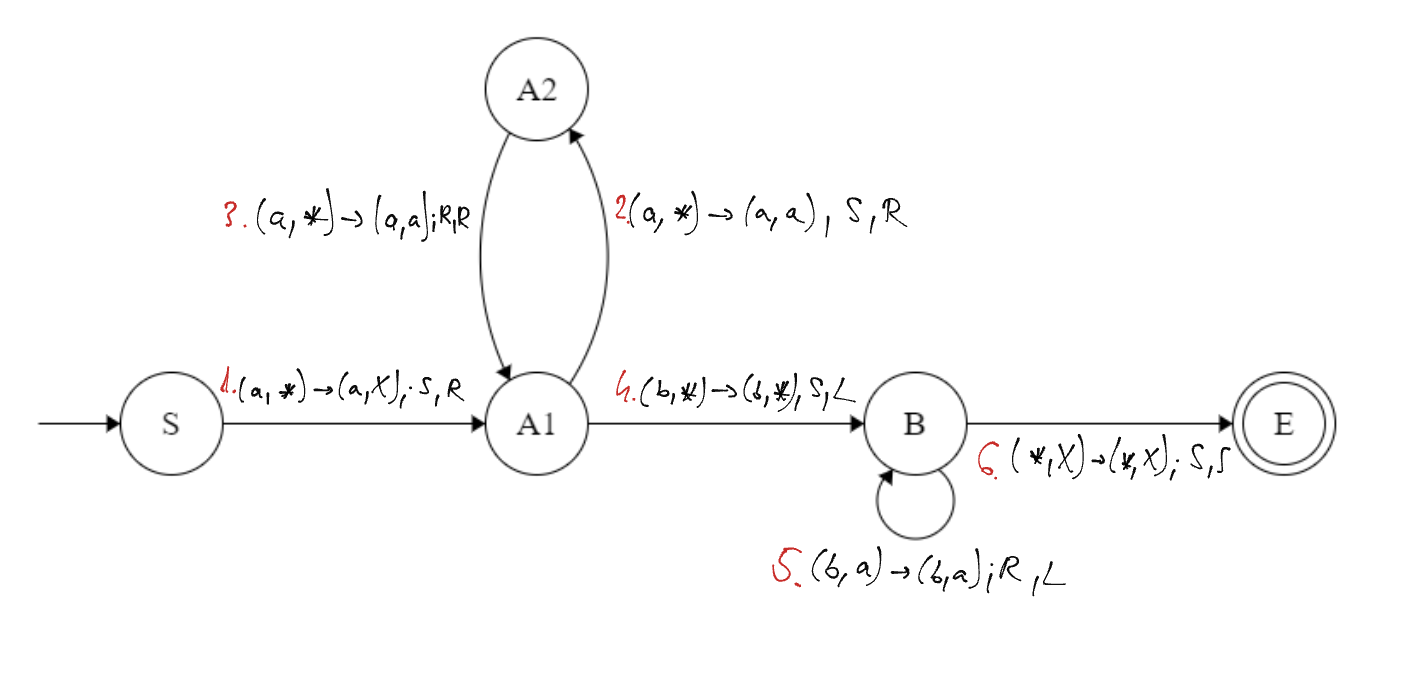
\includegraphics[width=\linewidth]{05/6_7_canvas.png}

\begin{itemize}
    \item Transition 1: We mark the beginning of the second tape with an $X$, so we don't fall off later.
    \item Transitions 2-3: For every $a$ character on the first tape we copy it twice to the second tape. Pay attention: in transition 2 the first head doesn't move, but in transition 3 it does.
    \item Transition 4: When the $a$'s are done and the $b$'s are coming we position the second head to the end of the copied $a$'s.
    \item Transition 5: We compare the number of $a$'s and $b$'s on the second and first tape. They have to be equal, which means that the original input had to have half as many $a$'s as $b$'s.
    \item Transition 6: If the first head reaches the end of the input at the same time the second head reaches the beginning of the second tape (marked with the $X$), it means that the number of $a$'s and $b$'s is correct and the word can be accepted.
\end{itemize}

b) Same as \ref{4f7}, but now we need to give a TM, instead of a PDA:

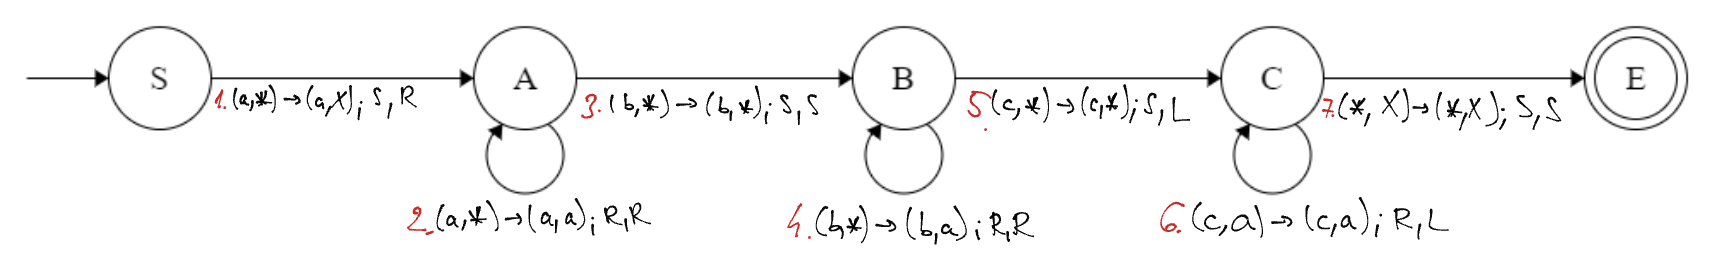
\includegraphics[width=\linewidth]{05/6_7_b_canvas.png}

\begin{itemize}
    \item Transition 1: We mark the beginning of the second tape with an $X$, so we don't fall off later.
    \item Transition 2: Copy the $a$'s to the second tape.
    \item Transition 3: Detect that the $b$'s are coming.
    \item Transition 4: Copy the $b$'s to the second tape, copy them as $a$'s since we only care about their collective numbers and this spares us one extra transition (similar to transition 6, but for a $b$).
    \item Transition 5: Detect that the $c$'s are coming.
    \item Transition 6: Compare the number of $a$'s and $b$'s = the number of $a$'s on the second tape to the number of $c$'s.
    \item Transition 7: If we run out of $a$'s and $c$'s at the same time it means that there were an equal number of them, so we can accept the input.
\end{itemize}

Important: Transition 1,3 and 5 enforce that $i,j,k \geq{} 1$.

c) 

The idea is to: Use 3 tapes, mark the beginning of the second and third tape. Copy the $a$'s to the first tape. Then step on the first $a$ on the second tape and run through the first tape copying all of the $b$'s to the third tape. Now step to the left on the second tape, and do the same for the next $a$, and do it until there are $a$'s left. When you reach the $X$ mark on the second tape, the third tape will contain $i \cdot j$ $b$'s. Now compare the number of $b$'s on the third tape to the remaining $c$'s on the first tape.

It is important to keep in mind that for an odd number of $a$'s the head on the first tape will be at the last $b$ (next to the $c$), while for an even number of $a$'s the head on the first thape will be at the first $b$ (not next to the $c$). Handle the latter case by moving the first head to the right until it sees a $c$.